%%%%%%%%%%%%%%%%%%%%%%%%%%%%%%%%%%%%%%%%%
% Simple Sectioned Essay Template
% LaTeX Template
%
% This template has been downloaded from:
% http://www.latextemplates.com
%
% Note:
% The \lipsum[#] commands throughout this template generate dummy text
% to fill the template out. These commands should all be removed when 
% writing essay content.
%
%%%%%%%%%%%%%%%%%%%%%%%%%%%%%%%%%%%%%%%%%

%----------------------------------------------------------------------------------------
%	PACKAGES AND OTHER DOCUMENT CONFIGURATIONS
%----------------------------------------------------------------------------------------
\documentclass[12pt]{report} 

\usepackage[pdftex]{hyperref} % Package for references
\hypersetup{
	breaklinks=true,
	pdfborder={0 0 0},
	pdfstartview={FitH},
	pdfpagemode={UseOutlines},
	pdftitle={},
	pdfauthor={},
	pdfsubject={},
	pdfkeywords={}
}

\usepackage{nameref}

\usepackage[footnotesize]{caption} % Adds the possibility to write text with the footnote size and sets a smaller size for the caption of images

\usepackage{geometry} % Required to change the page size to A4
\geometry{a4paper} % Set the page size to be A4 as opposed to the default US Letter

\usepackage{graphicx} % Required for including pictures

\usepackage[english]{babel}
\selectlanguage{english} % Sets to English the language of document

\usepackage[printonlyused]{acronym} %Deletes some blank pages

\usepackage[T1]{fontenc}	% Defines characters' type
\usepackage[latin1]{inputenc} 	% Defines admissible fonts

\usepackage{indentfirst} % Indents the first row of a paragraph

\usepackage{float} % Allows putting an [H] in \begin{figure} to specify the exact location of the figure
\usepackage{wrapfig} % Allows in-line images such as the example fish picture

\usepackage{lipsum} % Used for inserting dummy 'Lorem ipsum' text into the template

\usepackage{fancyvrb}

\usepackage{fancyhdr} % Used to customize the header and footer of pages, like page numbering

\usepackage{lastpage} % Used to obtain the number of pages

\usepackage{verbatim} % Used to insert block of comments

\usepackage{listings} % Package for listings
\lstset{
	tabsize=8,
	numbers=left,
	breaklines,
	breakatwhitespace,
	basicstyle=\scriptsize\ttfamily,
	keywordstyle=\bfseries,
	emphstyle=\ttfamily\itshape\underbar,
	showstringspaces=false,
	frame=single,
	captionpos=b,
	aboveskip=1em
}


\usepackage{enumitem}
\setlist{nosep} % Deletes the space before an items list and after

% Custom command to reset the page header and footer style
% This command must be called every time after a begin document is called or after a new chapter has begun
\newcommand{\setmyfancystyle}{
	\pagestyle{fancy}
	\thispagestyle{fancy}
	\fancyhead{}
	\fancyfoot{}
	\renewcommand{\headrulewidth}{0pt} % deletes the horizontal line in the page header
	\lhead{} \chead{} \rhead{}
	\lfoot{} \cfoot{}
	\rfoot{\thepage}
}
%-----------

\renewcommand{\rmdefault}{ppl}
\usepackage[scaled]{helvet}
\usepackage{courier}
\normalfont

\frenchspacing
\linespread{1.25} % Line spacing

%\setlength\parindent{0pt} % Uncomment to remove all indentation from paragraphs

\graphicspath{{Figures/}{../Figures/}} % Specifies the directory where pictures are stored

\usepackage{subfiles} % Allow to manage the document as different files (useful for working in two at the same time


%----------------------------------------------------------------------------------------
%	GLOSSARY
%----------------------------------------------------------------------------------------

\usepackage[nonumberlist, section, numberedsection, toc, style=altlist]{glossaries}	% Define the glossary as non numbered list, as numbered section (not chapter) and as an element into table of contents

\newglossaryentry{ws}
{
	name=WS,
	description={acronym for the website of the system}
}

\newglossaryentry{ma}
{
	name=MA,
	description={acronym for the mobile application}
}

\newglossaryentry{mockup}
{
	name=Mockup,
	text=mockup,
	plural=mockups,
	description={a simple graphical representation}
}


\makeglossaries

\begin{document}

%----------------------------------------------------------------------------------------
%	TITLE PAGE
%----------------------------------------------------------------------------------------

\begin{titlepage}

\newcommand{\HRule}{\rule{\linewidth}{0.5mm}} % Defines a new command for the horizontal lines, change thickness here

\center % Center everything on the page

\textsc{\huge \bf{Politecnico di Milano}}\\[0.5cm]
\textsf{\Large Department of Electronics, Information and Bioengineering}\\[0.25cm] % Major heading such as course name
\textsf{\large Master Degree course in Computer Science Engineering}\\[0.5cm] % Minor heading such as course title

\begin{figure}[h]
	\center 
\includegraphics[width = 3 cm]{Figures/PoliMi}
\end{figure}


\HRule \\
{\Huge \bfseries {Design Document (DD)} \\[0.2cm] \Large {myTaxiService}}\\ % Title of your document
\HRule \\[1cm]

\begin{figure}[h]
	\center 
\includegraphics[width=2cm]{Figures/logo3}
\end{figure}


\begin{flushleft}
	\large \textit{Instructor:} Prof. Elisabetta Di Nitto \\[0.5cm]

\begin{minipage}{0.45\textwidth}
\begin{flushleft} \large
\emph{Authors:}\\
Luca Costanzo\\
Simone Disabato
\end{flushleft}
\end{minipage}
~
\begin{minipage}{0.45\textwidth}
\begin{flushright} \large
\emph{Code:} \\
789038\\
852863
\end{flushright}
\end{minipage}\\[1 cm]

\end{flushleft} 

{\large \today}\\ % Date, change the \today to a set date if you want to be precise

%\includegraphics{Logo}\\[1cm] % Include a department/university logo - this will require the graphicx package

\vfill % Fill the rest of the page with whitespace

\end{titlepage}
\newpage

%----------------------------------------------------------------------------------------
%	TABLE OF CONTENTS
%----------------------------------------------------------------------------------------

\tableofcontents % Include a table of contents

\newpage % Begins the essay on a new page instead of on the same page as the table of contents 

%----------------------------------------------------------------------------------------
%	CHAPTERS
%----------------------------------------------------------------------------------------

%Introduction
\subfile{Chapters/chapter1_Introduction}
%Architectural Design
\subfile{Chapters/chapter2_ArchitecturalDesign}
%Algorithm Design
%\providecommand{\mainpath}{..} % Command to retrieve the path of the main file. It must be defined before documentclass.

\documentclass[\mainpath/main]{subfiles}
\begin{document}

\chapter{Algorithm Design}
\label{algorithm_design}

% Command to be executed after the starting of every chapter
\setmyfancystyle
% ----------------

In this chapter the most interesting algorithm of myTaxiService are presented using pseudo-code (every developer can easily translate the pseudo-code into the desired programming language). In addition this pseudo-code is referred to an object-oriented programming language, like C++ or Java (the reader can think about the equivalent algorithm in non object-oriented programming language like C, so he has to create manually all the object data structures, the objects himself and he has to define a way to manage and save all the created objects).\\
The meaning of word \textit{interesting}, used above to define the algorithms which we will present in this chapter, is the following: a characteristic and unique algorithm, used to implement a specific functionalities of this system. For instance, an algorithm to manage the backup of the database can be very complicated in describing the policies, the exceptions and the situations when execute its, but it is a common algorithm for all the systems that store data into a database.\\
\\
In this chapter the algorithms analysed are the following:
\begin{itemize}
	\item the city's areas creations and management;
	\item the queue's management;
	\item all the algorithms used to handle the special situation which occur when no cabmen are available in the area where the ride (which the Ride Allocator is now assigning) starting position is.\\
\end{itemize}

\section{Map and Areas' Creation Algorithms}
\label{AlgorithmDesign:MapAreaAlgorithms}

\textit{Premise. The system has, at its disposal, an XML document that describes the city and its streets. The structure of the document is shown below and it is the following: first there are the four extreme coordinates in order to create a rectangle which contains all the city's area (if the borders of the city are irregular the rectangle's area is bigger than the city's area), then all the streets are listed with the name and two coordinates. In fact, with this two points the street can be represent as the line that joins these two points.}

\begin{figure}[ht!]
	\centering
\fbox{\begin{minipage}{0.8\textwidth}
		\footnotesize
		\textit{\hspace*{1cm}  <City> \\
		\hspace*{2cm} <Extreme Coordinates>\\
		\hspace*{3cm} <WestX> \textellipsis </WestX>\\
		\hspace*{3cm} <SouthY> \textellipsis </SouthY>\\
		\hspace*{3cm} <EastX> \textellipsis </EastX>\\
		\hspace*{3cm} <NorthY> \textellipsis </NorthY>\\
		\hspace*{2cm} </Extreme Coordinates>\\
		\hspace*{2cm} <Streets>\\
		\hspace*{3cm} <Street direction = \textquotedblleft H\textquotedblright>\\
		\hspace*{4cm} <Name> \textellipsis </Name>\\
		\hspace*{4cm} <Left Position>\\
		\hspace*{5cm} <X> \textellipsis </X>\\
		\hspace*{5cm} <Y> \textellipsis </Y>\\
		\hspace*{4cm} </Left Position>\\
		\hspace*{4cm} <Right Position>\\
		\hspace*{5cm} <X> \textellipsis </X>\\
		\hspace*{5cm} <Y> \textellipsis </Y>\\
		\hspace*{4cm} </Right Position>\\
		\hspace*{3cm} </Street>\\
		\hspace*{3cm} [\textellipsis]\\
		\hspace*{3cm} <Street> [\textellipsis] </Street>\\
		\hspace*{2cm} </Streets>\\
		\hspace*{1cm} </City>}
\end{minipage}}
\caption{Structure of XML document that describes the city.}
\end{figure}

\textit{For each street an attribute direction is defined: the value H indicates a horizontal road so the two coordinates are the left and the right, while the value V indicates a vertical road so the two coordinates are the high and the low.}\\
\\
When the system starts the map creation it first creates the areas objects. The idea is simple: starting form the Northwest angle of the map it create square areas of side 1.5 kilometres\footnote{Due to the city is not perfectly rectangular, this algorithm can create some areas that cover lands out of the city borders. This is not a relevant problem in memory usage.}.\\

\fbox{\begin{minipage}{0.8\textwidth}
		\hspace*{0.5 cm} MapCreator.createMap(WestX , SouthY , EastX , NorthY);\\[0.1cm]
		\hspace*{0.5 cm} {\color{green} horizontalSectors} = (EastX - WestX) / {\color{red} 1.5} + {\color{red} 1};\\
		\hspace*{0.5 cm} {\color{green} verticalSectors} = (NorthY - SouthY) / {\color{red} 1.5} + {\color{red} 1};\\
		\hspace*{0.5cm} {\color{cyan} \textit{for}} {\color{green} i} = {\color{red} 0} -> {\color{green} verticalSectors} {\color{cyan} \textit{then}}\\
		\hspace*{1.5 cm} {\color{cyan} \textit{for}} {\color{green} j} = {\color{red} 0} -> {\color{green} horizontalSectors} {\color{cyan} \textit{then}}\\
		\hspace*{2.5cm} MapCreator.createArea(j , i);
	\end{minipage}}\\[0.5cm]
	
We point out two aspect of the code shown above: first, in the calculus of the number of areas, both in vertical and horizontal, we sum one at the result to count the final area which has a size less than the fixed dimension (1.5 km); second, the notation used in the \textit{for} indicates a cycle of \textit{n} interactions where \textit{n} is equal to the value written at the right of the edge.\\
\\
Now, the objects of type \textit{area} are created, but they do not contain any street. The algorithm used to add the streets is simple: for each street into the XML document (we suppose we have a parser which gives all the streets found into the document as an object), the belonging area is the one where the first coordinates is in. To avoid strange situations where a street is assigned to an area even if only a small part belongs to the area\footnote{This situation happens, for instance, when the left coordinate is near the right bound of the area and it has an horizontal direction.} an additional parameter \textit{CORRECTOR} is defined. The parameter assumes one value into the interval [0,1] (the value we have chosen is 0.7). To assign a horizontal street (for the vertical ones is similar) the rules are the following (the map can consider as a grid):
\begin{itemize}
	\item the row into the map is exactly the one where the left coordinate is in;
	\item the column into the map is exactly the one where the left coordinate is in if and only if its position is not near the right bound (on the other hand the street is assigned to the next area on the right). Called \textit{size} the dimension of an area and \textit{x} the distance between the coordinate and the starting of the area \textit{start}, the coordinate is near the area's right bound if:
	\begin{center}
		$ x \textgreater start + size * CORRECTOR $;
	\end{center}
\end{itemize}
Now the algorithm is shown by restricting the use of chain invocations in order to make the algorithm easy to read.\\

\fbox{\begin{minipage}{0.8\textwidth}
		{\color{blue} \textit{//We suppose we have an iterator between the streets, given by the parser. From now we'll call it parserIt.}}\\[0.3cm]
		\hspace*{0.3cm} {\color{cyan} \textit{while}} ({\color{green} parserIt}.hasNext()) {\color{cyan} \textit{then}}\\
		\hspace*{1.3cm} {\color{green} street} = {\color{green} parserIt}.next();\\
		\hspace*{1.3cm} {\color{green} x} = {\color{green} street}.firstCoordinate().getX();\\
		\hspace*{1.3cm} {\color{green} y} = {\color{green} street}.firstCoordinate().getY();\\
		\hspace*{1.3cm} {\color{green} row} = ({\color{green} x} - WestX) / {\color{red} 1.5};\\
		\hspace*{1.3cm} {\color{green} col} = (NorthY - {\color{green} y}) / {\color{red} 1.5};\\
		\hspace*{1.3cm} {\color{cyan} \textit{if}} ( {\color{green} street}.type().equalTo(\textquoteleft V\textquoteright) \&\& checkY(y , row)) {\color{cyan} \textit{then}}\\
		\hspace*{2.3cm} {\color{green} row} = {\color{green} row} + {\color{red} 1};\\
		\hspace*{1.3cm} {\color{cyan} \textit{else if}} ( {\color{green} street}.type().equalTo(\textquoteleft H\textquoteright) \&\& checkX(x, col)) {\color{cyan} \textit{then}}\\
		\hspace*{2.3cm} {\color{green} col} = {\color{green} col} + {\color{red} 1};\\
		\hspace*{1.3cm} Map.getArea(row,col).addStreet(street);
	\end{minipage}}\\[0.5cm]
Now the two methods checkY and checkX are shown.\\
Both the methods have a boolean return type and try to verify it is needed to increase by one the calculated area (see above for the reasons). The parameter are different according to the type of the street: for a vertical road are required the y-part of the first coordinate and the calculated row while for a horizontal road the x-part of the first coordinate and the calculated column.\\

\fbox{\begin{minipage}{0.8\textwidth}
		\hspace*{0.5cm} boolean checkY (double y , int row) \textbraceleft \\
		\hspace*{1.5cm} {\color{green} start} = NorthY - {\color{green} row} * {\color{red} 1,5};\\
		\hspace*{1.5cm} {\color{cyan} \textit{if}} ({\color{green} y} \textgreater ({\color{green} start} + {\color{red} 1,5} * CORRECTOR)) {\color{cyan} \textit{then}}\\
		\hspace*{2,5cm} {\color{cyan} \textit{return}} \textbf{true};\\
		\hspace*{1,5cm} {\color{cyan} \textit{return}} \textbf{false};\\
		\hspace*{0.5cm} \textbraceright \\
		\\
		\hspace*{0.5cm} boolean checkX (double x , int col) \textbraceleft \\
		\hspace*{1.5cm} {\color{green} start} = EastX + {\color{green} col} * {\color{red} 1,5};\\
		\hspace*{1.5cm} {\color{cyan} \textit{if}} ({\color{green} x} \textgreater ({\color{green} start} + {\color{red} 1,5} * CORRECTOR)) {\color{cyan} \textit{then}}\\
		\hspace*{2,5cm} {\color{cyan} \textit{return}} \textbf{true};\\
		\hspace*{1,5cm} {\color{cyan} \textit{return}} \textbf{false};\\
		\hspace*{0.5cm} \textbraceright
	\end{minipage}}\\[0.5cm]
	
This algorithm generates a first division of the city and its streets into the areas. The algorithm is not perfect and does not consider same particular situations as restricted-traffic zones or busy roads. To improve the quality of the city areas the administrators are able to move some streets between two areas. The administrators are supposed to decide to change a street with some criteria, so no checks are performed on those action.\\
Finally, the final version of the city is saved on the database, even if a representation is maintained into the Ride Allocator (to be precisely the constructed version). 

\section{Queue Creator Algorithms}
\label{AlgorithmDesign:QueueCreatorAlgorithms}

The Queue Creator is a subcomponent of the Ride Allocator\footnote{see the \autoref{ArchitecturalDesign:provider} for a complete description.}.\\
The queues' creation is an iterative process performed at the Ride Allocator creation and initialization. After the definition of the map and its areas, the Queue Creator is involved to create one queue into each area.\\

\fbox{\begin{minipage}{0.8\textwidth}
		\hspace*{3cm}  {\color{cyan} \textit{forall}} Area {\color{green} a} {\color{cyan} \textit{in}} Map {\color{cyan} \textit{then}}\\
		\hspace*{4cm}   {\color{green} a}.createQueue();
	\end{minipage}}\\[0.5cm]

The \textit{createQueue} method is defined into the class Area: it is able to create one object \textit{queue} if and only if it has never created another queue yet. This definition does not require a Factory Method\footnote{see the \autoref{ArchitecturalDesign:design_patterns} for a definition.} pattern, because exists only one type of queue and no other types can be designed in future. In addition, an exception will be thrown if the method is called when a queue already exists\footnote{In a non object oriented programming language this error can be notified using a return value of the method createQueue. However this method can be called only by the Queue Creator, that is involved only once.}.\\
\\
Into the database this method has no effects because no driver is waiting at the creation of the queues that are empty.

\section{Queue Manager Algorithms}
\label{AlgorithmDesign:QueueManagerAlgorithms}

The Queue Manager has two main algorithms: one to add a driver to a queue by a position and the other one to update a queue (moving down or remove a driver).\\
When a driver needs to be added to a queue, first the Queue Manager uses the Google Maps APIs to find the street by the position, then identify the area by a method into the Map component. (not shown here). At last is able to add the driver to the correct queue in the last position.\\

\fbox{\begin{minipage}{0.8\textwidth}
				\hspace*{0.5cm} void addDriver (Driver d , Position pos) \textbraceleft \\
				\hspace*{1.5cm} {\color{green} street} = GoogleMaps.getStreetByPosition(pos);\\
				\hspace*{1.5cm} {\color{green} area} = Map.getArea (street);\\
				\hspace*{1.5cm} {\color{green} area}.enqueue(d);
				\hspace*{1.5 cm} {\color{blue} \textit{//The method enqueue does not involves any methods into the DBMS. The System Controller, when asks for a driver adding, also call a similar function into the DBMS.}}\\
				\hspace*{0.5cm} \textbraceright
	\end{minipage}}\\[0.5cm]
	
When a driver has to be removed from the queue, the Queue Manager gives a specific method which is so simple: it removes only the first element into the desired area's queue. In addition, the method also gives the possibilities to move the driver from the first position to the last one by a flag. The changes need to be stored into the database, so the Ride Allocator, at his return, passes to the System Controller the results of the operations and the DBMS is able to correctly update the queue information. Hence, the Queue Manager only updates the queues, but it does not save any data.\\

\fbox{\begin{minipage}{0.8\textwidth}
		\hspace*{0.5cm} void moveDriver (Area a , boolean moveDown) \textbraceleft \\
		\hspace*{1.5cm} {\color{green} driver} = {\color{green} area}.removeFirstElement();\\
		\hspace*{1.5cm} {\color{cyan} \textit{if}} (moveDown) {\color{cyan} \textit{then}}\\
		\hspace*{2.5cm} {\color{green} area}.enqueue(driver);\\
		\hspace*{0.5cm} \textbraceright
	\end{minipage}}\\[0.5cm]

\section{Ride Assignment Algorithm}
\label{AlgorithmDesign:RideAssignmentAlgorithm}

The ride are assigned by the Ride Allocator and inside that, by the Allocator subcomponent. The allocator can access to the Map and, as consequence, to the areas and to the related queues. When the System Controller involves the Ride Allocator to assign a driver to an imminent ride, it delegates also the possibilities to pass through the Client and Users Handler in order to communicate with the drivers, then it waits for the results (they will be saved on the database).\\
The method used to assign a ride has only two parameters, the starting and the destination position. In an object oriented programming language this method will be defined using the overload principle to allows the possibility to use as starting position either a position or an address. For the destination position the method can accept only addresses. In this description we suppose that the method receives only addresses\footnote{in the version with position, the reader can see the \autoref{AlgorithmDesign:QueueManagerAlgorithms} to have an idea about the \textquotedblleft conversion\textquotedblright from a position to an address.}.\\
The first passage for the algorithm is to find the correct area associated to the address and in this case the methods of the Map are used, as in \autoref{AlgorithmDesign:QueueManagerAlgorithms}. Afterwards, the Ride Allocator calls the first driver in the queue and waits for his answer one minute.\footnote{In the RASD document the driver has been supposed to answer immediately to a call, but to avoid some infinite waiting of the system (for instance for connecting problems on the driver's device) we define now a timer after which the cabman's answer is consider to be a deny.} Here, there are two possibilities: first the driver accepts, so the Ride Allocator immediately removes the driver from the queue and returns to the System Controller; else the driver denies, so the Ride Allocator move the driver to the bottom of the queue and then asks to the next driver into the queue.\\
In both the possible cases the Ride Allocator has a list (the real implementation of this list is not given here) where save the key information about the ride that it is now assigning: so the detected area and the sequence of driver involved. The answers of each driver are not needed because only the last driver in the list has accepted the ride.\\

\fbox{\begin{minipage}{0.8\textwidth}
		\hspace*{0.5cm} \textit{list} assignRide (Address start, Address destination, \textit{linkToClientAndUsersHandler} handler) \textbraceleft \\
		\hspace*{1.5cm} {\color{green} area} = Map.getArea(start);\\
		\hspace*{1.5cm} {\color{green} listToReturn}.add(area);\\
		\hspace*{1.5 cm} {\color{cyan} \textit{do}} \\
		\hspace*{2.5cm} {\color{green} driver} = {\color{green} area}.removeFirstElement();\\
		\hspace*{2.5cm} {\color{green} area}.enqueue(driver);\\
		\hspace*{2.5cm} {\color{blue} //Above the driver is re-added to the queue}\\
		\hspace*{2.5cm} {\color{green} listToReturn}.add(driver);\\
		\hspace*{2.5cm} {\color{green} accepted} = {\color{green} handler}.ask(destination, \textit{timer value});\\
		\hspace*{1.5cm} {\color{cyan} \textit{while}} ({\color{green} accepted} == \textbf{false});\\
		\hspace*{1.5cm} {\color{green} area}.removeLastDriver();\\ 
		\hspace*{0.5cm} \textbraceright
	\end{minipage}}\\[0.5cm]

\textit{Observation: the method ask of the handler asks to a cabman if he want to drive in a ride to a certain destination. The second parameter is the maximum time that the driver has to answer: if the timer expires the method return false (the notification of this event to the cabman is then handled by the Client and Users Handler)}.

\section{Special Algorithms}
\label{AlgorithmDesign:special}

In this section will be given only an accurate description of the algorithms used to administrate the special situation that occur when in some area there is no driver into the queue.\\
In the previous section, the algorithm that assign a ride does not consider this possibility. In some objected oriented languages this can be accepted and the special algorithm is invoked by an exception. In alternative is possible define a more exhaustive control flow that call the special algorithms into an if condition.\\
The system does not allow an human-defined sequence of near areas to be called, so in this situation the first area chosen to find a driver will be randomly selected among the areas closest to the one where the starting position is in.\\
After the choice of the next area the algorithm shown in \autoref{AlgorithmDesign:RideAssignmentAlgorithm} is called to find a driver for the ride. Obviously, if also this area has no available driver, a new area will be chosen to search a driver who is waiting.\\

\section{Conclusion}
\label{AlgorithmDesign:conclusion}

In this chapter all the algorithms have been presented without consider the possibility to receive more than one rides to be assigned at the same time. If the two or more rides are in different areas, no problem occurs even if the algorithms are called in parallel.\\
A precisation about the case that happen when two contemporaneous rides start from the same area is required. Calling in parallel the shown algorithm to assign the rides may lead to inconsistent and undesired situations. This problem can be easily solved by the introduction of synchronization strategies. The implementation of this strategies will not be discussed here, but to have an idea a possible (partial) solution is to have more than one thread to execute ride assignment. When the Ride Allocator is waiting for the driver's answer, it can accepts new requests on an other thread and, if the same area is involved the following driver in the queue will be involved, and so on. Note that this description does not describes all the aspects concerning the synchronization: for instance what happen if the first thread need another driver at the same time of the second one? In addition, if there is only one driver into the queue and he rejects the first ride, the system has to asks to him before enter into the special mode (this is a very strange and rarely case).







\end{document}
% User Interface Design
%\providecommand{\mainpath}{..} % Command to retrieve the path of the main file. It must be defined before documentclass.

\documentclass[\mainpath/main]{subfiles}
\begin{document}

\chapter{User Interfaces Design}
\label{UIDesign}

% Command to be executed after the starting of every chapter
\setmyfancystyle
% ----------------

In this chapter are shown the main \glspl{mockup} of myTaxiService, due to present the graphical user interfaces of the system for each functionality. All the \glspl{mockup} are displayed with an accurate description to prevent misunderstanding and to recall the functionality.\\

\section{Registration/Login}
\label{UI:RegistrationAndLogin}
When an user connects to the WS or opens the MA, the first screens is the login page. For both the versions, there is a button to redirect to the registration page, if the user is not registered yet.\\
The figure \ref{UI:loginWS} is the WS version where the registration button is made by a link on the phrase \textquotedblleft Not Registered yet? Click here\textquotedblright. At the same time the user can insert his credentials into the specific boxes.\\
The figure \ref{UI:loginMA} is the corresponding \gls{mockup} for the mobile application: at the application opening the user can inserts his credentials or clicks on the registration button.\\

\clearpage

\begin{figure}[ht!]
	\centering
	\begin{minipage}[t]{0.45\textwidth}
		\centering
		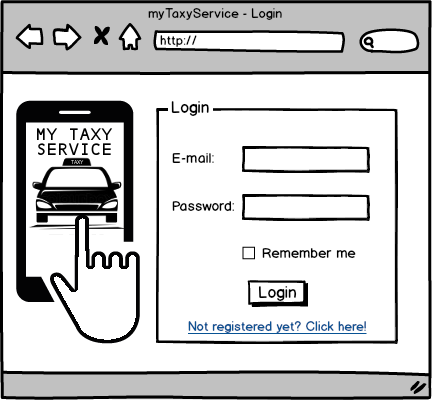
\includegraphics[width = \linewidth] {mockups/Login_WS}
		\caption{Login page into website.}
		\label{UI:loginWS}
	\end{minipage}
	\hspace{0.05 cm}
	\begin{minipage}[t]{0.45\linewidth}
		\centering
		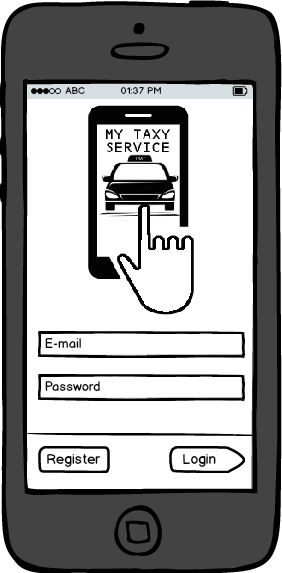
\includegraphics[height = 8cm] {mockups/Login_MA}
		\caption[Login page into mobile application.] {\scriptsize Login page into mobile application.}
		\label{UI:loginMA}
	\end{minipage}
\end{figure}

A non registered user has to enrol into the system, so he clicks on the corresponding button and he is redirected to that page. The figures \ref{UI:registrationWS} and \ref{UI:registrationMA} shows the \glspl{mockup} for this: into the \gls{ma} the box labels are written into them and disappears when the user fills in; into the \gls{ws} the labels are shown near the corresponding one.\\

\begin{figure}[ht!]
	\centering
	\begin{minipage}[t]{0.45\textwidth}
		\centering
		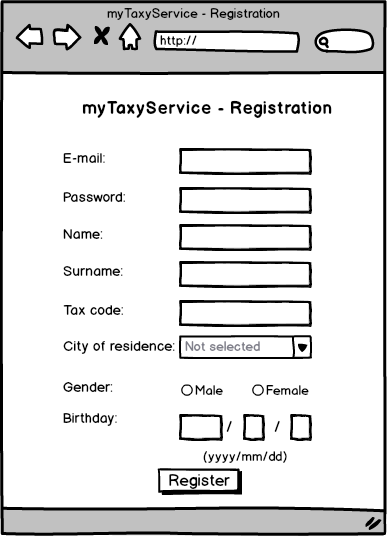
\includegraphics[width = \linewidth] {mockups/Registration_WS}
		\caption{Registration page into website.}
		\label{UI:registrationWS}
	\end{minipage}
	\hspace{0.05 cm}
	\begin{minipage}[t]{0.45\linewidth}
		\centering
		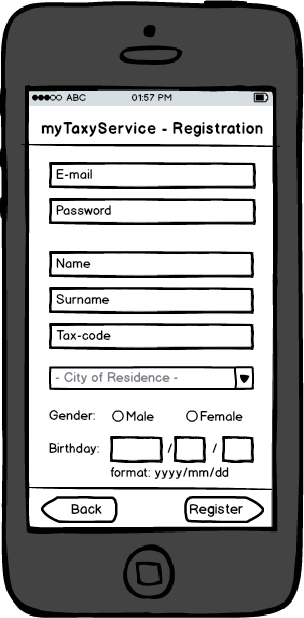
\includegraphics[height = 8cm] {mockups/Registration_MA}
		\caption[Registration page in mobile application.] {\scriptsize Registration page in mobile application.}
		\label{UI:registrationMA}
	\end{minipage}
\end{figure}

\section{Personal Information Management}
\label{UI:PersonalInformationManagement}
The figures \ref{UI:managePersonalInformationWS} and \ref{UI:managePersonalInformationMA} show the mockups for the  management of personal information.\\
The only information that can be modified are the email, the password and the city of residence. In both the myTaxiService's versions the other information are shown into a non-modifiable boxes (so they have a different color, typically grey, to mark this property).

\begin{figure}[ht!]
	\centering
	\begin{minipage}[t]{0.45\textwidth}
		\centering
		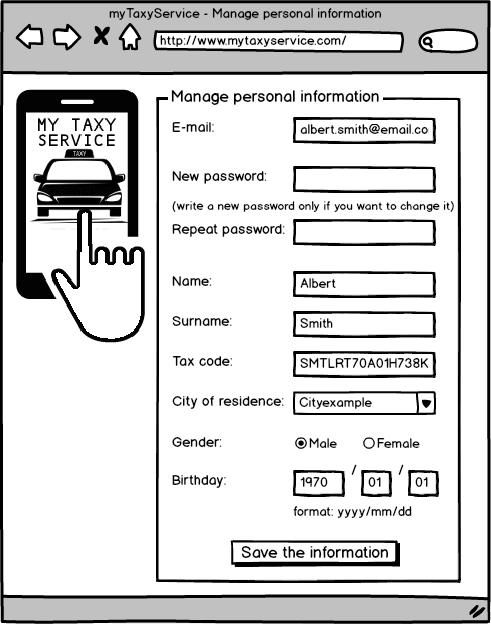
\includegraphics[width = \linewidth] {mockups/ManagePersonalInformation_WS}
		\caption{Personal Information Management page into website.}
		\label{UI:managePersonalInformationWS}
	\end{minipage}
	\hspace{0.05 cm}
	\begin{minipage}[t]{0.45\linewidth}
		\centering
		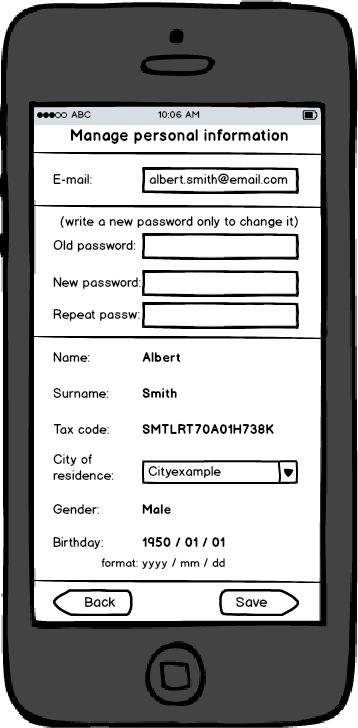
\includegraphics[height = 9cm] {mockups/ManagePersonalInformation_MA}
		\caption{Personal Information Management page in mobile application.}
		\label{UI:managePersonalInformationMA}
	\end{minipage}
\end{figure}

\clearpage

\section{Driver functionalities}
\label{UI:DriverFunctionalities}
The functionalities reserved for the cab-men are developed only for the \gls{ma} version of myTaxiService: the reasons are explained in \autoref{ArchitecturalDesign:preamble}. When a cab-man has to notify the system that it is starting his work shift or he has ended a ride, so he is now waiting for a new ride, he uses the Start Waiting Time functionality that is shown in figure \ref{UI:startWaitingTime}: the displayed position is calculated by GPS.\\

\begin{figure}[ht!]
	\centering
	\begin{minipage}[t]{0.45\textwidth}
		\centering
		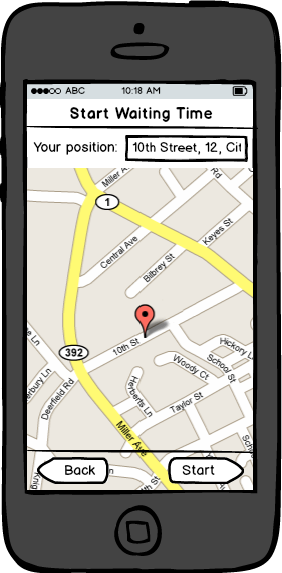
\includegraphics[height = 9 cm]{mockups/StartWaitingTime}
		\caption{The Start Waiting Time page.}
		\label{UI:startWaitingTime}
	\end{minipage}
	\hspace{0.05 cm}
	\begin{minipage}[t]{0.45\linewidth}
		\centering
		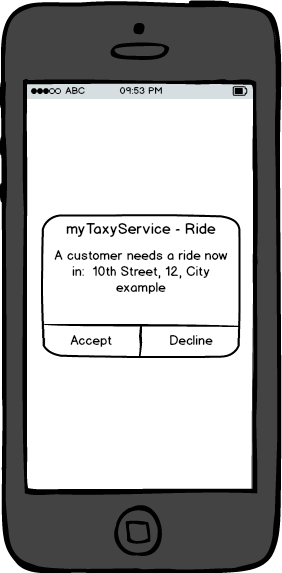
\includegraphics[height = 9 cm]{mockups/AcceptDenyRide}
		\caption[The request for a ride to a driver page.]{The request for a ride page.}
		\label{UI:acceptDenyRide}
	\end{minipage}
\end{figure}

During this period, the system can asks the driver to make a ride, so in figure \ref{UI:acceptDenyRide} it is shown the screen for this request.\\
At last, in figure \ref{UI:workshift} there is a mockup for the page where the driver can modify his workshifts. He can add, modify or remove them. The page where the driver can see his workshifts is not displayed, but it is similar to the shown one, without the modification symbols.\\
\\
\\

\begin{figure}[ht!]
	\centering
	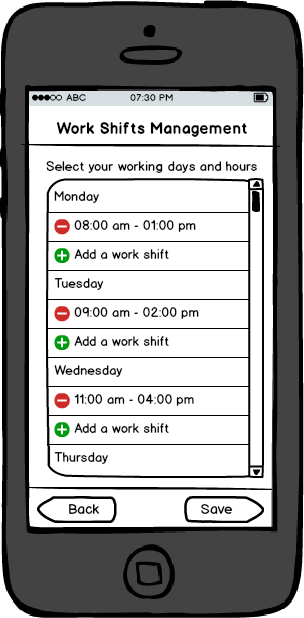
\includegraphics[height = 8 cm]{mockups/WorkShiftsManagement}
	\caption{The workshifts management page.}
	\label{UI:workshift}
\end{figure}

\section{Zerotime Ride}
\label{UI:ZerotimeRide}
When a user asks for a zerotime ride, he has to insert the starting and the destination positions (the first one can be calculated by the GPS) and then to confirm the request.\\
In the \gls{ma} this sequence of operations is performed with three screens (\glspl{mockup} in figures \ref{UI:zerotimeMA1}, \ref{UI:zerotimeMA2} and \ref{UI:zerotimeMA3}), while into the \gls{ws} it is used only one screen split into the correspondent sections, shown in figure \ref{UI:zerotimeWS}.

\begin{figure}[ht!]
	\centering
	\begin{minipage}[t]{0.4\textwidth}
		\centering
		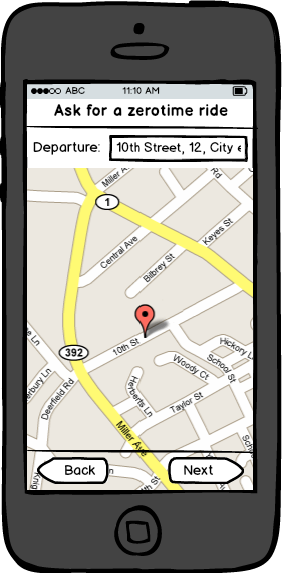
\includegraphics[height = 8 cm]{mockups/AskForZerotimeRide_MA_1}
		\caption[Zerotime ride request part1 into mobile application.]{Zerotime ride request into mobile application: starting position insert (manually or by GPS) page.}
		\label{UI:zerotimeMA1}
	\end{minipage}
	\hspace{1 cm}
	\begin{minipage}[t]{0.40\linewidth}
		\centering
		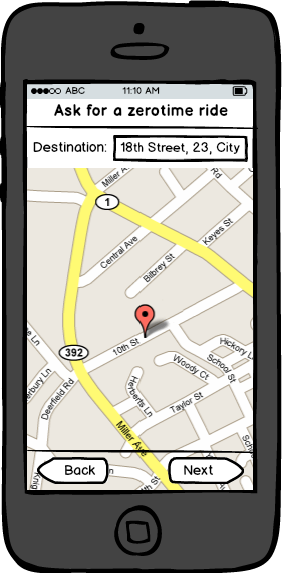
\includegraphics[height = 8 cm]{mockups/AskForZerotimeRide_MA_2}
		\caption[Zerotime ride request part2 into mobile application.]{Zerotime ride request into mobile application: destination position insert page.}
		\label{UI:zerotimeMA2}
	\end{minipage}
\end{figure}

\begin{figure}[ht!]
	\centering
	\begin{minipage}[t]{0.4\textwidth}
		\centering
		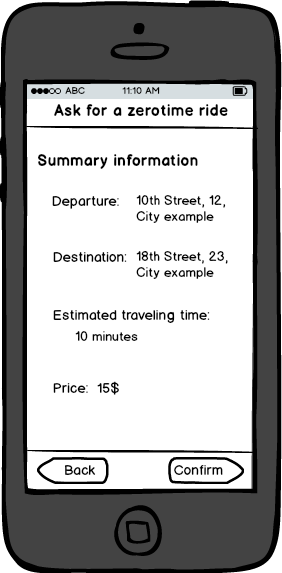
\includegraphics[height = 8.5 cm]{mockups/AskForZerotimeRide_MA_3}
		\caption[Zerotime ride request part3 into mobile application.]{Zerotime ride request into mobile application: confirmation page.}
		\label{UI:zerotimeMA3}
	\end{minipage}
	\hspace{1 cm}
	\begin{minipage}[t]{0.40\linewidth}
		\centering
		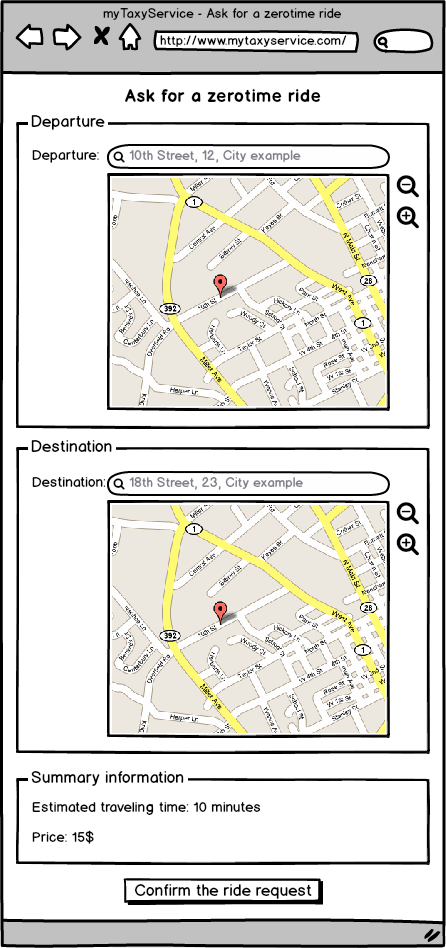
\includegraphics[height = 8.5 cm]{mockups/AskForZerotimeRide_WS}
		\caption[Zerotime ride request into website.]{Zerotime ride request into website page.}
		\label{UI:zerotimeWS}
	\end{minipage}
\end{figure}

\clearpage

\section{Future Ride}
\label{UI:FutureRide}
When a user desires to book a future ride, he has to insert the starting and the destination positions (the first one can be calculated by the GPS), the departure (both the date and the time) and then to confirm the request.\\
In the \gls{ma} this sequence of operations is performed with three screens (\glspl{mockup} in figures \ref{UI:futuretimeMA1}, \ref{UI:futuretimeMA2} and \ref{UI:futuretimeMA3}), while into the \gls{ws} it is used only one screen split into the correspondent sections, shown in figure \ref{UI:futuretimeWS}.\\
In both the \gls{ma} and the \gls{ws}, the departure inserting is made with a pop-up that uses the apposite operative system functionalities to insert the dates (for example a computer OS can use a calendar for dates and a box for time, while a mobile OS can use a dropdown list or something that slides following the finger's touch).\\

\begin{figure}[ht!]
	\centering
	\begin{minipage}[t]{0.4\textwidth}
		\centering
		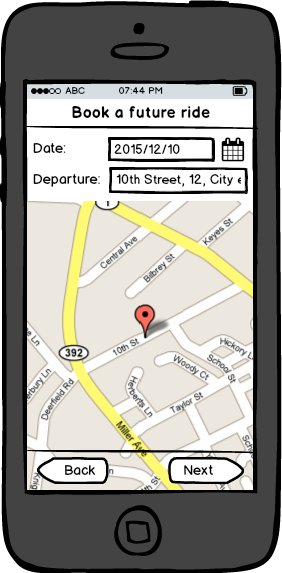
\includegraphics[height = 9 cm]{mockups/BookFutureRide_MA_1}
		\caption[Future ride request part1 into mobile application.]{Future ride request into mobile application: departure starting position insert (manually or by GPS) page.}
		\label{UI:futuretimeMA1}
	\end{minipage}
	\hspace{1 cm}
	\begin{minipage}[t]{0.40\linewidth}
		\centering
		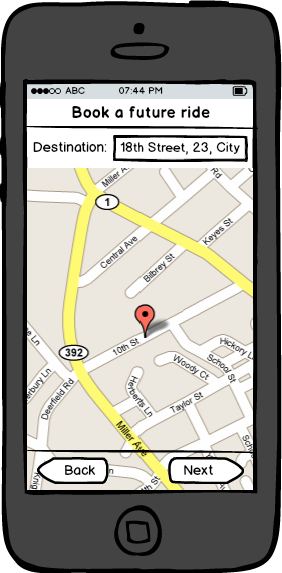
\includegraphics[height = 9 cm]{mockups/BookFutureRide_MA_2}
		\caption[Future ride request part2 into mobile application.]{Future ride request into mobile application: destination position insert page.}
		\label{UI:futuretimeMA2}
	\end{minipage}
\end{figure}

\begin{figure}[ht!]
	\centering
	\begin{minipage}[t]{0.4\textwidth}
		\centering
		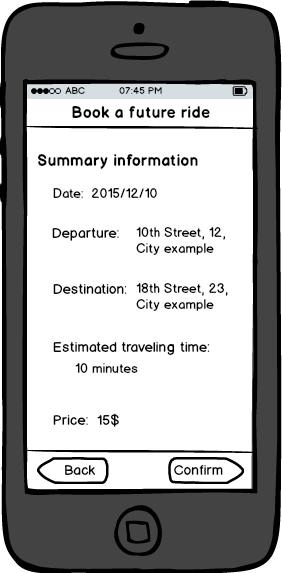
\includegraphics[height = 9 cm]{mockups/BookFutureRide_MA_3}
		\caption[Future ride request part3 into mobile application.]{Future ride request into mobile application: confirmation page.}
		\label{UI:futuretimeMA3}
	\end{minipage}
	\hspace{1 cm}
	\begin{minipage}[t]{0.40\linewidth}
		\centering
		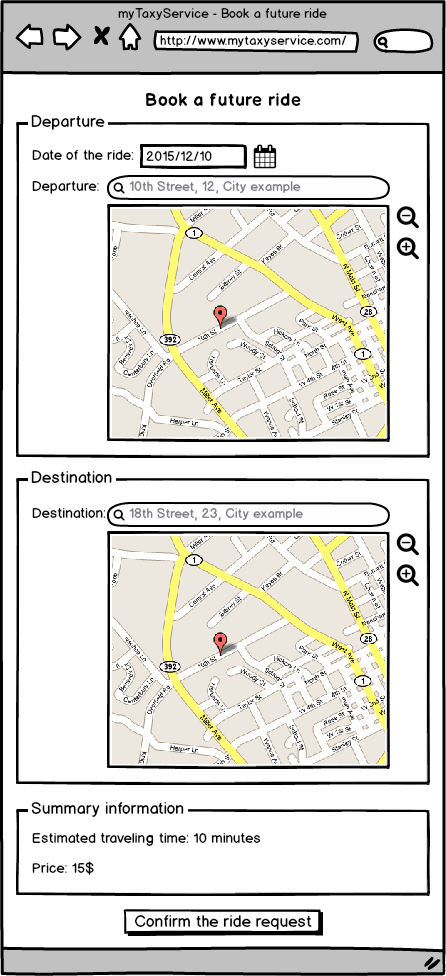
\includegraphics[height = 9 cm]{mockups/BookFutureRide_WS}
		\caption[Future ride request into website.]{Future ride request into website page.}
		\label{UI:futuretimeWS}
	\end{minipage}
\end{figure}

\section{Other User Functionalities}
\label{UI:OtherUserFunctionalities}
myTaxiService gives other useful functionalities to the users.\\
In \gls{ma} there are two screens: in figure \ref{UI:reservationMA1} the users can see all his reservation split into two sections, one for the future reservation (they can be edited) and one, at the bottom, for a list of the past rides; in figure \ref{UI:reservationMA2} the user can edit a specific reservation (either the departure or the positions can be modified) that it was selected in the previous page by a click on the \textquotedblleft edit, delete\textquotedblright  button.\\

\clearpage

\begin{figure}[ht!]
	\centering
	\begin{minipage}[t]{0.4\textwidth}
		\centering
		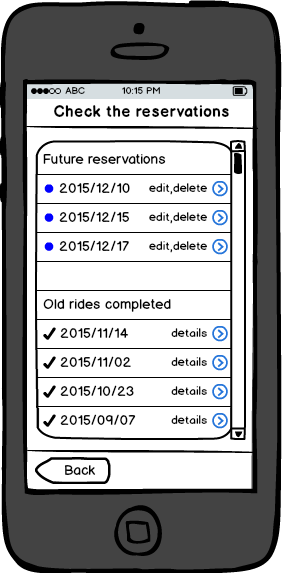
\includegraphics[height = 8 cm]{mockups/CheckReservations_MA_1}
		\caption[View reservation into mobile application.]{The view reservations page into mobile application.}
		\label{UI:reservationMA1}
	\end{minipage}
	\hspace{1 cm}
	\begin{minipage}[t]{0.40\linewidth}
		\centering
		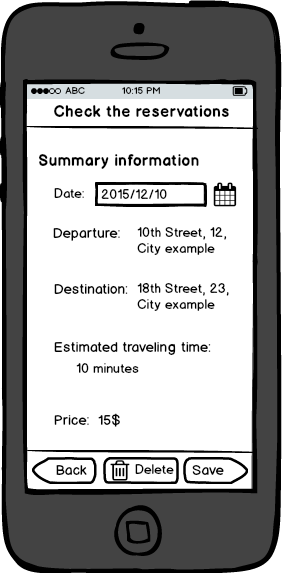
\includegraphics[height = 8 cm]{mockups/CheckReservations_MA_2}
		\caption[Modify reservations into mobile application.]{The page where a reservation can be modified or be cancelled into mobile application.}
		\label{UI:reservationMA2}
	\end{minipage}
\end{figure}

In \gls{ws} the same operations can be performed into the same page, displayed in figure \ref{UI:reservationWS}.

\begin{figure}[ht!]
	\centering
	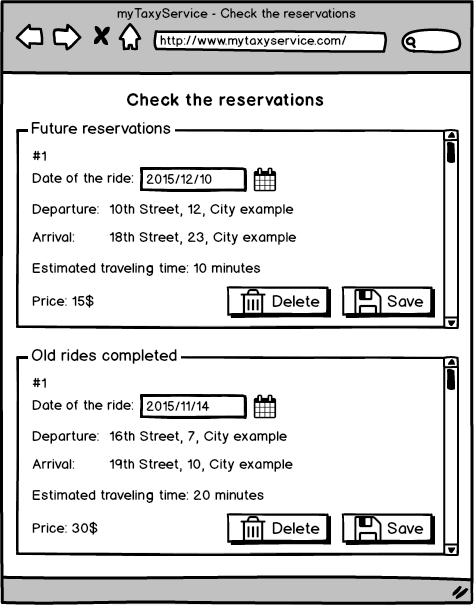
\includegraphics[height = 7.5 cm]{mockups/CheckReservations_WS}
	\caption[Check reservation into website.]{The check reservation page into page.}
	\label{UI:reservationWS}
\end{figure}

\clearpage

Finally, the user can received some alerts regarding, for instance, the assignment of the ride for which he asked for. The alerts can also be a general information, related to some problems of the service or to a strike.\\
The corresponding screen for the \gls{ma} and the \gls{ws} are shown, respectively, in figures \ref{UI:alertsMA} and \ref{UI:alertsWS}.

\begin{figure}[ht!]
	\centering
	\begin{minipage}[t]{0.4\textwidth}
		\centering
		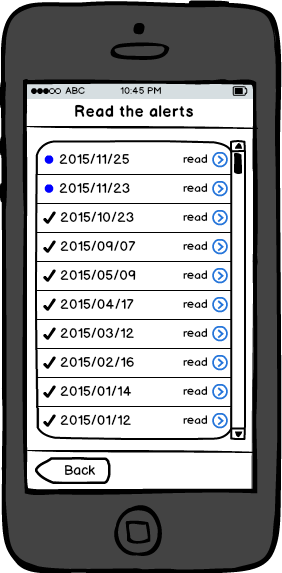
\includegraphics[height = 7 cm]{mockups/ReadAlerts_MA}
		\caption[Read the alerts into mobile application.]{The alerts page into mobile application.}
		\label{UI:alertsMA}
	\end{minipage}
	\hspace{0.5 cm}
	\begin{minipage}[t]{0.40\linewidth}
		\centering
		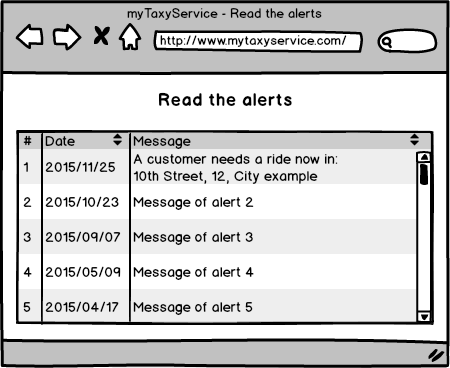
\includegraphics[width = \linewidth]{mockups/ReadAlerts_WS}
		\caption[Read the alerts into website.]{The alerts page into website.}
		\label{UI:alertsWS}
	\end{minipage}
\end{figure}

%End of chapter
\end{document}
%Requirements traceability
%\providecommand{\mainpath}{..} % Command to retrieve the path of the main file. It must be defined before documentclass.

\documentclass[\mainpath/main]{subfiles}
\begin{document}

\chapter{Requirements Traceability}
\label{RequirementsTraceability}
This chapter explains how the functional requirements from the Requirements Analysis And Specification Document (RASD) have been designed and described in this Design Document (DD).\\
Every section of this chapter refers to a functional requirement.

\section{Registration}
The section \ref{RASD:requirements:Registration} of the RASD describes the registration functionality. A visitor can register himself to myTaxyService only if he's new to the system, i.e. doesn't exist a user with the same tax code.\\
In the DD we have satisfied this functional requirement, we have described the sequence of actions in the Sequence Diagram of \autoref{ArchitecturalDesign:SD_Registration} and represented the user interface to register both via \gls{ma} and \gls{ws} in \autoref{UI:RegistrationAndLogin}.

\section{Login}
The section \ref{RASD:requirements:Login} of the RASD describes the login functionality. A visitor can login into myTaxyService only if he's registered.
In the DD we have satisfied this functional requirement, we have described the sequence of actions in the Sequence Diagram of \autoref{ArchitecturalDesign:SD_Login} and represented the user interface to login both via \gls{ma} and \gls{ws} in \autoref{UI:RegistrationAndLogin}.

\section{Personal Information Management}
The section \ref{RASD:requirements:PersonalInformationManagement} of the RASD describes the personal information management functionality. A logged user can modify some of his personal information: the e-mail, the password and the city of residence.\\
In the DD we have satisfied this functional requirement, we have described the sequence of actions in the Sequence Diagram of \autoref{ArchitecturalDesign:SD_ProfileManagement} and represented the user interface to manage personal information both via \gls{ma} and \gls{ws} in \autoref{UI:PersonalInformationManagement}.

\section{Ask for a Zerotime Ride}
The sections \ref{RASD:requirements:ZerotimeReservationMA} and \ref{RASD:requirements:ZerotimeReservationWS} of the RASD describe the functionality of asking for a zerotime ride both via \gls{ma} and via \gls{ws}. A logged user can ask for a zerotime ride.\\
In the DD we have satisfied this functional requirement, we have described the sequence of actions in the Sequence Diagram of \autoref{ArchitecturalDesign:SD_Zerotime} and represented the user interface to ask for a zerotime ride both via \gls{ma} and \gls{ws} in \autoref{UI:ZerotimeRide}.

\section{Book a Future Ride}
The section \ref{RASD:requirements:FutureReservation} of the RASD describes the functionality of booking a future ride both via \gls{ma} and via \gls{ws}. A logged user can book a future ride.\\
In the DD we have satisfied this functional requirement, we have described the sequence of actions in the Sequence Diagram of \autoref{ArchitecturalDesign:SD_FutureRide} and represented the user interface to book a future ride both via \gls{ma} and \gls{ws} in \autoref{UI:FutureRide}.

\section{Accept or Deny a Ride}
The section \ref{RASD:requirements:ZerotimeReservationMA} of the RASD also describes within the functionality of the Driver to accept or deny a ride, via \gls{ma}. A logged driver can accept or deny a request for a ride when he receives it.\\
In the DD we have satisfied this functional requirement and we have represented the user interface to accept or deny a ride via \gls{ma} in \autoref{UI:DriverFunctionalities}.

\section{Start Waiting Time}
The section \ref{RASD:requirements:StartWaitingTime} of the RASD describes the functionality of starting the waiting time via \gls{ma}. A logged driver notifies the system that he's available in an area and waiting for a ride and he is added to the queue of the area.\\
In the DD we have satisfied this functional requirement, we have described the sequence of actions in the Sequence Diagram of \autoref{ArchitecturalDesign:SD_StartWaitingTime} and represented the user interface to start waiting time via \gls{ma} in \autoref{UI:DriverFunctionalities}.

\section{Work Shifts Management}
The section \ref{RASD:requirements:WorkShiftsManagement} of the RASD describes the functionality of management of the work shifts via \gls{ma}. A logged driver can add or delete a work shift in the week days.\\
In the DD we have satisfied this functional requirement, we have described the sequence of actions in the Sequence Diagram of \autoref{ArchitecturalDesign:SD_WorkShiftsManagement} and represented the user interface to manage the work shifts via \gls{ma} in \autoref{UI:DriverFunctionalities}.

\section{Check the Reservations}
The section \ref{RASD:requirements:CheckReservations} of the RASD describes the functionality of checking the reservations (both zerotime and future rides) both via \gls{ma} and via \gls{ws}. A logged user can view the his reservations, modify the date or cancel them.\\
In the DD we have satisfied this functional requirement, we have described the sequence of actions in the Sequence Diagram of \autoref{ArchitecturalDesign:SD_CheckReservation} and represented the user interface to check the reservations both via \gls{ma} and \gls{ws} in \autoref{UI:OtherUserFunctionalities}.

\section{Read the Alerts}
The section \ref{RASD:requirements:ReadAlerts} of the RASD describes the functionality of reading the received alerts both via \gls{ma} and via \gls{ws}. A logged user can only view his alerts, he cannot edit them.\\
In the DD we have satisfied this functional requirement and we have represented the user interface to read the alerts both via \gls{ma} and \gls{ws} in \autoref{UI:OtherUserFunctionalities}.



\end{document}
%Info
\subfile{Chapters/OtherInfo}


\end{document}
